\documentclass[border=2pt]{standalone}
\usepackage{tikz}
\usetikzlibrary{matrix,positioning,arrows.meta,arrows}

\tikzset{
mymat/.style={
  matrix of nodes,
  nodes in empty cells,
  text height=2.5ex,
  text depth=0.75ex,
  text width=3.25ex,
  align=center,
  column sep=-\pgflinewidth
  }
}
\tikzset{
  rows/.style 2 args={
    sub@rows/.style={row ##1 column #2/.style={nodes={rectangle,draw=black}}},
    sub@rows/.list={#1}
  },
  box/.style 2 args={
    sub@box/.style={rows={#1}{##1}},
    sub@box/.list={#2}
  }
}
\begin{document}

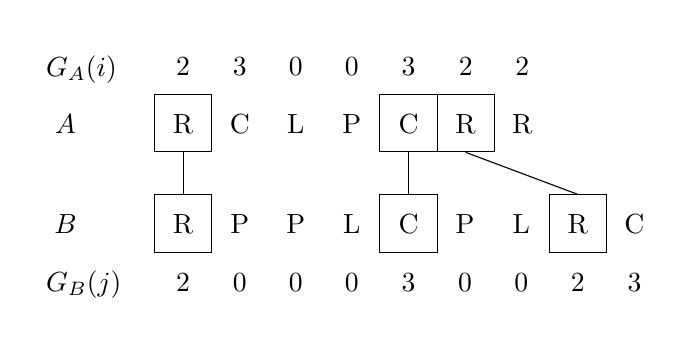
\begin{tikzpicture}[>=latex]
\matrix[mymat,anchor=west,
    box={2}{1, 5, 6}]
at (0,0) 
(mat1)
{
2 & 3 & 0 & 0 & 3 & 2 & 2 \\
R & C & L & P & C & R & R \\
};
\matrix[mymat,anchor=west,
    box={1}{1, 5, 8}]
at (0,-2) 
(mat2)
{
R & P & P & L & C & P & L & R & C \\
2 & 0 & 0 & 0 & 3 & 0 & 0 & 2 & 3 \\
};

\matrix[mymat]
at (-1, 0)
(mat1Text)
{
   $G_A(i)$ \\
   $A$ \\
};

\matrix[mymat]
at (-1, -2)
(mat2Text)
{
   $B$ \\
   $G_B(j)$ \\
};

\begin{scope}
\draw[]
  (mat1-2-1.south) -- (mat2-1-1.north);
\draw[]
  (mat1-2-5.south) -- (mat2-1-5.north);
\draw[]
  (mat1-2-6.south) -- (mat2-1-8.north);
\end{scope}
\end{tikzpicture}

\end{document}